\documentclass[conference]{IEEEtran}
\usepackage{tikz}
\usepackage{graphicx}
\usepackage{float}

\usetikzlibrary
	{ arrows
	, positioning
	, fit
	, shapes
	, calc
	}

\begin{document}

\title{The Hadoop Framework}

\author{\IEEEauthorblockN{Stephen O'Brien}
\IEEEauthorblockA{Cork Institute of Technology}
}

\maketitle
\suppressfloats

\begin{abstract}
This report details an overview of Hadoop, its components and architecture.
\end{abstract}

% creates the second title. It will be ignored for other modes.
\IEEEpeerreviewmaketitle



\section{Introduction}
Hadoop is a framework for data processing at a large scale, born from two papers 
released by Google - \emph{MapReduce: Simplified Data Processing on Large Clusters} \cite{mapreduce} and \emph{The Google File System} \cite{gfs}. 
The Google File System paper outlines the architecture for Googles proprietary distributed filesystem, used for large distributed applications. 
The MapReduce paper outlines a programming model for processing large datasets.

\section{Hadoop Architecture}
At a high level Hadoop consists of two layers, a compute layer, \emph{YARN} (Yet Another Resource Negotiator) and a storage layer, \emph{HDFS} (Hadoop Distributed File System). \emph{YARN} provides API's for request work to be scheduled on the cluster. These API's are generally consumed by frameworks such as \emph{Apache Spark} or \emph{MapReduce}, these frameworks then expose higher level API's allowing users to write applications and not have to worry about interacting directly with \emph{YARN}.

The storage layer, \emph{HDFS}, was built for very large files, 100GB's/TB's or larger and was built to run on commodity hardware. It manages large files by splitting them up into a sequence of blocks and storing the blocks across machines in a cluster of storage nodes.

Above the compute and storage layers sits the frameworks which use \emph{YARN}'s API's to schedule work across the cluster. \emph{MapReduce} is one of these frameworks, but there are many more - Apache Spark, Hive, Pig, to name a few. See Figure ~\ref{highlevelarch} for a simple visual overview.

\begin{figure}[ht]
\centering
\scalebox{0.5}{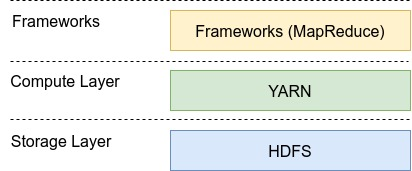
\includegraphics[width=\textwidth]{images/HadoopHighLevelArch.jpeg}}
\caption{High Level Overview of Hadoop Architecture}
\label{highlevelarch}
\end{figure}

\subsection{HDFS}
\emph{HDFS} is a distributed file system, designed to handle large datasets. \emph{HDFS} embraces the idea that a write-once read-many data processing pattern is the most efficient. Typically within Hadoop an analysis of a dataset would use the whole of, or most of, the dataset so for \emph{HDFS} the read time of the entire dataset is more important than the latency of reading the first item in the dataset. 

The architecture of a HDFS comprises of a single \emph{NameNode} and multiple \emph{DataNodes}, NameNodes can also be federated, whereby multiple NameNodes work independently but use the same underlying DataNodes. The NameNode manages the filesystem namespace, it uses \emph{inodes} to represent files, directories and related metadata. File contents are split into blocks, which are replicated and stored across multiple DataNodes. The NameNode also manages this mapping of file contents to blocks across DataNodes. A read of file data from a HDFS client will first request block locations of the file from the NameNode, once the locations are received the client uses these locations to read blocks from the nearest DataNode \cite{hdfs}. This read operation is outlined in Figure \ref{clientread}.

\begin{enumerate}
\item Client requests block location information from the NameNode.
\item The NameNode responds giving the closes DataNode to the client for each block requested.
	\item \begin{enumerate}
     \item One of the block locations was local, the client requests this directly.
     \item Another block was store on a different DataNode on another rack, the client also requests this directly.
   \end{enumerate}
\end{enumerate}


\begin{figure}[ht]
\centering
\scalebox{0.5}{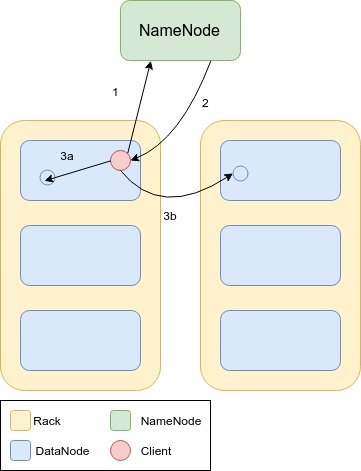
\includegraphics[width=\textwidth]{images/clientread.jpg}}
\caption{High Level Overview of HDFS Architecture}
\label{clientread}
\end{figure}

Loss of a NameNode means complete loss of all files that NameNode was managing as it is the single source which knows how to reconstruct files from their constituent blocks. One way to prevent this is to run a \emph{secondary NameNode} \cite{secnamenode} which takes snapshots of the primary NameNode's state over time, if the primary NameNode fails the secondary can take over.

\subsection{YARN}
YARN is Hadoop's cluster resource management system. It provides an API for working with cluster resources, this allows management of resources to be abstracted away from developers when using frameworks such as MapReduce - MapReduce exposes a higher level API using YARN underneath to manage resources. YARN consists of two daemons - a per-cluster \emph{ResourceManager} and a set of \emph{NodeManagers} \cite{yarn}.

A NodeManager runs on every node in the cluster and are responsible for monitoring resource availability, tracking and alerting on faults, and managing the lifecycle of \emph{containers}. Containers execute application specific processes within bounded resources, YARN can run containers and limit resources as processes directly or by using Linux \emph{cgroups}.

\begin{figure}[ht]
\centering
\scalebox{0.5}{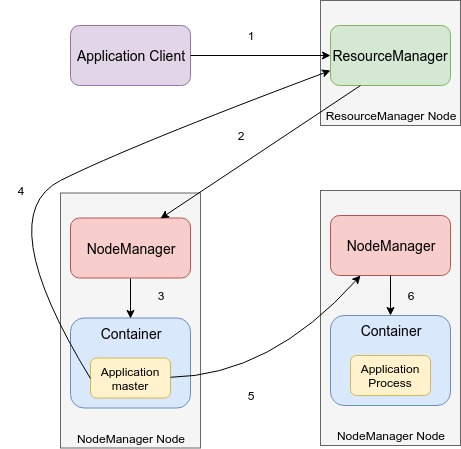
\includegraphics[width=\textwidth]{images/yarn.jpg}}
\caption{YARN application lifecycle overview}
\label{yarn}
\end{figure}


\subsection{MapReduce}
The MapReduce paper \cite{mapreduce} introduced a programming model for data generation and data processing. The model defines a computation which takes a set of key/value pairs as input and produces a set of key/value pairs as output.
This computation is composed of two different functions, \emph{Map} and \emph{Reduce}. \emph{Map} takes a key value pair as input and produces a set of \emph{intermediate} key/value pairs. These inermediate key/value pairs are processed by the \emph{MapReduce} library, which groups all values associated with each key and sends them to the \emph{Reduce} function. \emph{Reduce} takes the key and its set of values and produces zero or more outputs, depending on what the writer of the \emph{Reduce} function wanted to learn from the data.

\emph{MapReduce} is a framework in Hadoop implementing the above programming model. Within this framework the unit of work is called a \emph{job}, it abstracts job resource management from writers of \emph{MapReduce} applications, calling the YARN API internally to have it schedule and manage jobs. Hadoop executes a job by splitting it into \emph{tasks} of which there are two kinds - map tasks and reduce tasks. The input of a job is divided into splits \cite{mapreduce}, there is one map task per split. This makes it highly parallelizable, more splits equals less processing time. However, if splits are too small the overhead of managing them will dominate job execution time.

Split sizes are generally the same size as the block size in HDFS (whose default is 128MB) \cite{hdfs}. The advantage being the block size is the largest slie of input guaranteed to be on an node. If the split size spanned two or more blocks it would be highly unlikely any single node had all those blocks.

Hadoop tries to run map tasks on a node where the input to the task resides, this helps to reduce cluster bandwidth usage as data does not have to be transferred between nodes to feed map tasks - the higher the data locality the less data has to be copied from node to node. Sometimes this is not possible, so the job scheduler will try to use a node on the same rack (a rack is the physical machine nodes are located on) - failing that it will try off rack nodes. The point of this process is to try to keep data locality as high as possible when executing map tasks.

Once a map task is complete, it writes the output to the local filesystem and not to HDFS, the map outputs are intermediate and will be discarded once the reduce task consumes them. For reduce, there is generally no data locality , the input is usually the output of all map tasks (there can be partitioning of reduce tasks also).

\section{Conclusion}
The conclusion goes here.


\begin{thebibliography}{1}
\bibitem{mapreduce}
Jeffrey Dean and Sanjay Ghemawat, \emph{MapReduce: Simplified Data Processing on Large Clusters}, December 2004.

\bibitem{gfs}
Sanjay Ghemawat, Howard Gobioff, and Shun-Tak Leung, \emph{The Google File System}, October 2003.

\bibitem{hdfs}
Konstantin Shvachko, Hairong Kuang, Sanjay Radia, Robert Chansler, \emph{The Hadoop Distributed File System},  May 2010.

\bibitem{secnamenode}
https://hadoop.apache.org/docs/stable/hadoop-project-dist/hadoop-hdfs/HdfsUserGuide.html.

\bibitem{yarn}
Vavilapalli et al., \emph{Apache Hadoop YARN: Yet Another Resource Negotiator}, October 2013.

\end{thebibliography}

\end{document}


